\documentclass[preprint,11pt,authoryear]{elsarticle}
%% Use the option review to obtain double line spacing
%% \documentclass[authoryear,preprint,review,12pt]{elsarticle}
\usepackage[onehalfspacing]{setspace}
\usepackage[a4paper, total={14cm, 19cm}]{geometry}

\usepackage{url}
\usepackage[T1]{fontenc}
\usepackage[algo2e,linesnumbered,ruled]{algorithm2e} 
\usepackage{appendix}
\usepackage{tabularx}       % automatic column width
\usepackage{mathtools}  
%\usepackage{amssymb}
%\usepackage{amsmath}
\usepackage{amsfonts}       % mathbb
\usepackage{xfrac}          % slanted fractions
\usepackage{bm}             % bold greeks 
\usepackage [autostyle, english = american]{csquotes} % left and right opening quotes with "
\usepackage{wrapfig}        % text flows around image
\usepackage{array}          % Needed for custom column types
\usepackage{xcolor}
\colorlet{added}{blue!80!black} 
\usepackage{setspace}       % for controlled interline
% \usepackage{lineno}
\usepackage{enumitem}
%\usepackage{caption}
%\usepackage[labelfont=sf]{subcaption}
%\captionsetup{subrefformat=parens,font=footnotesize}
%\subcaptionsetup[figure]{textfont=sf,position=bottom}
\usepackage{./eqndefns-left} % For checking the display equation width and equation environment definitions 
%\usepackage{graphicx}
%% For including figures, graphicx.sty has been loaded in
%% elsarticle.cls. If you prefer to use the old commands
%% please give \usepackage{epsfig}

\journal{Computers \& Operations Research}

\begin{document}

\begin{frontmatter}

%% Title, authors and addresses

%% use the tnoteref command within \title for footnotes;
%% use the tnotetext command for theassociated footnote;
%% use the fnref command within \author or \affiliation for footnotes;
%% use the fntext command for theassociated footnote;
%% use the corref command within \author for corresponding author footnotes;
%% use the cortext command for theassociated footnote;
%% use the ead command for the email address,
%% and the form \ead[url] for the home page:
%% \title{Title\tnoteref{label1}}
%% \tnotetext[label1]{}
%% \author{Name\corref{cor1}\fnref{label2}}
%% \ead{email address}
%% \ead[url]{home page}
%% \fntext[label2]{}
%% \cortext[cor1]{}
%% \affiliation{organization={},
%%            addressline={}, 
%%            city={},
%%            postcode={}, 
%%            state={},
%%            country={}}
%% \fntext[label3]{}

\title{} %% Article title

%% use optional labels to link authors explicitly to addresses:
%% \author[label1,label2]{}
%% \affiliation[label1]{organization={},
%%             addressline={},
%%             city={},
%%             postcode={},
%%             state={},
%%             country={}}
%%
%% \affiliation[label2]{organization={},
%%             addressline={},
%%             city={},
%%             postcode={},
%%             state={},
%%             country={}}

\author{} %% Author name

%% Author affiliation
\affiliation{organization={},%Department and Organization
            addressline={}, 
            city={},
            postcode={}, 
            state={},
            country={}}

%% Abstract
\begin{abstract}
%% Text of abstract
Abstract text.
\end{abstract}

%%Graphical abstract
\begin{graphicalabstract}
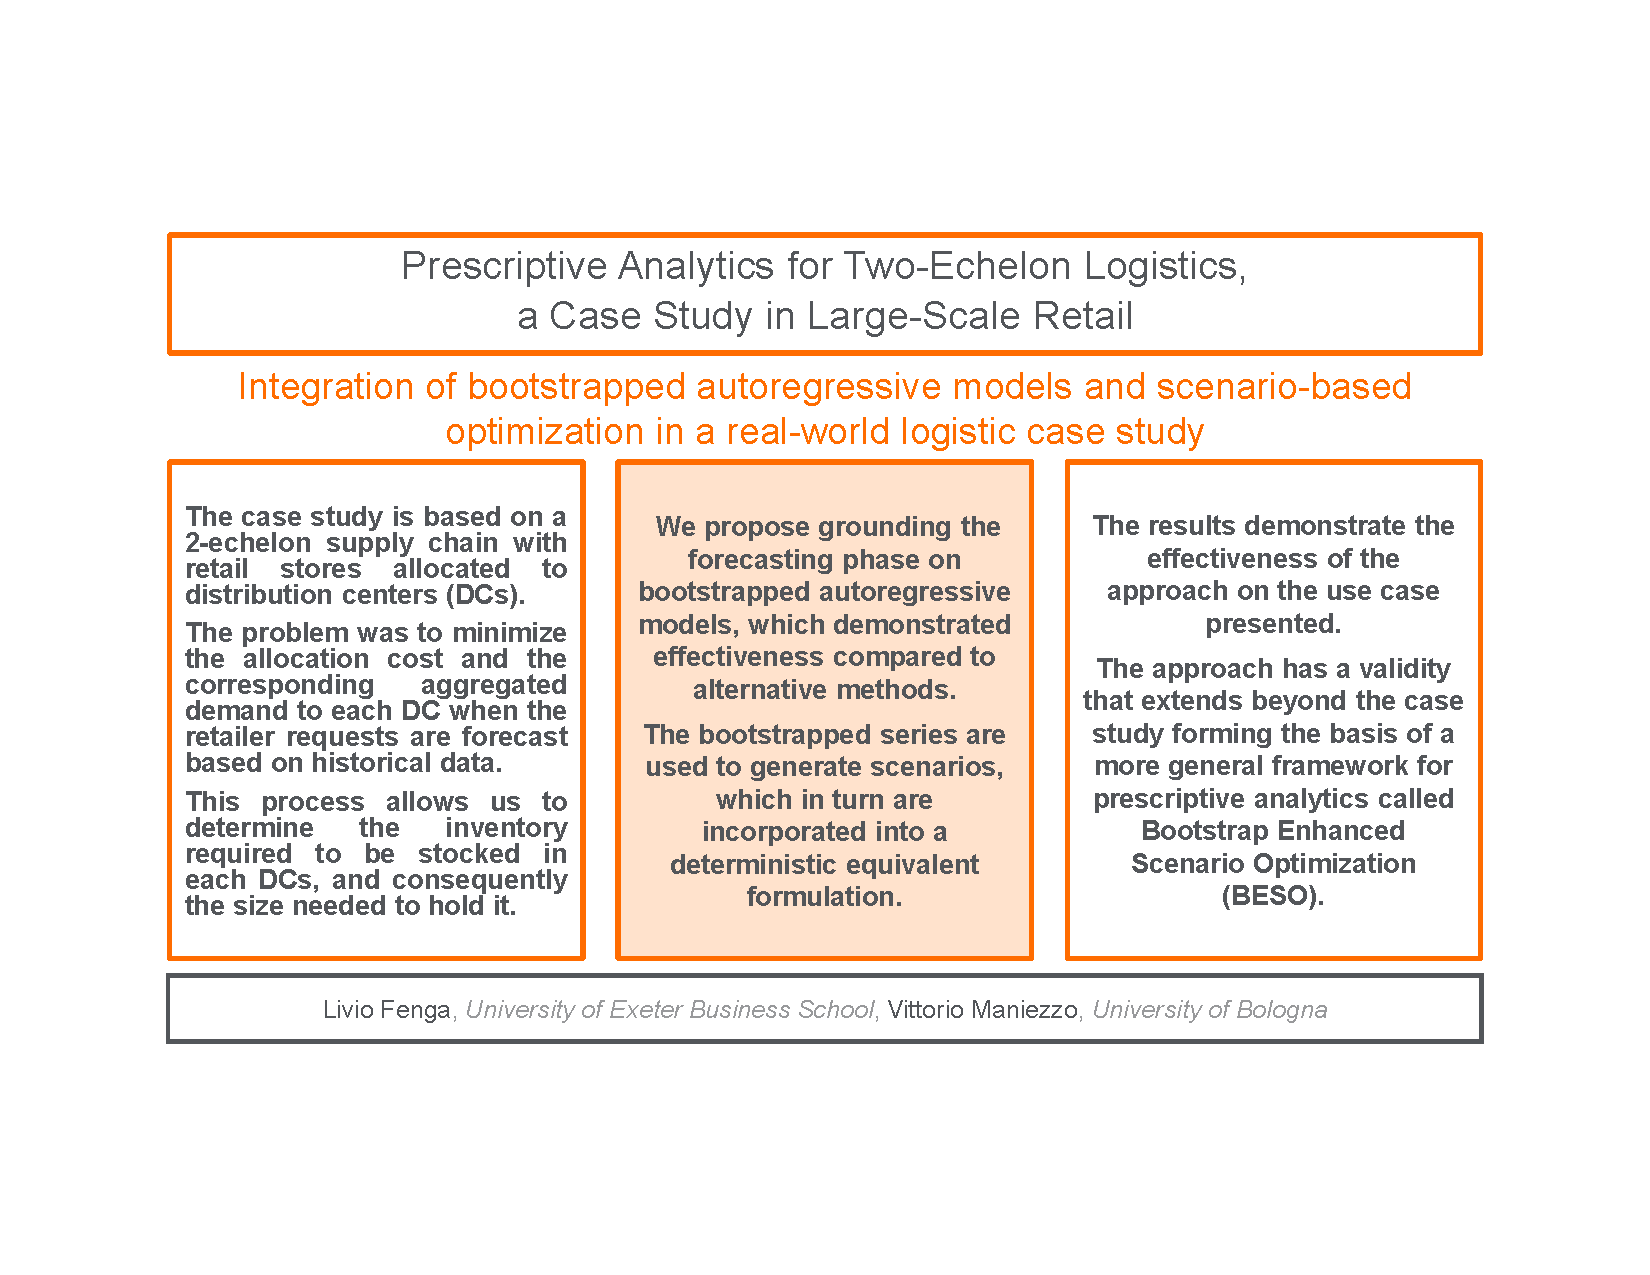
\includegraphics[width=\linewidth]{Visual-abstract}
\end{graphicalabstract}

%%Research highlights
\begin{highlights}
	\item A new framework for integrating time series forecasting into stochastic programming.
	\item Maximum Entropy Bootstrap with bagging for forecasting short logistic time series.
	\item Bootstrap distributions for deterministic equivalent scenario generation.
	\item Predictive analytics for warehouse sizing.
	\item Real-world 2-echelon logistics case study.
\end{highlights}

%% Keywords
\begin{keyword}
%% keywords here, in the form: keyword \sep keyword

%% PACS codes here, in the form: \PACS code \sep code

%% MSC codes here, in the form: \MSC code \sep code
%% or \MSC[2008] code \sep code (2000 is the default)

\end{keyword}

\end{frontmatter}

%% Add \usepackage{lineno} before \begin{document} and uncomment 
%% following line to enable line numbers
%% \linenumbers

%% main text
%%

%% Use \section commands to start a section
\section{Example Section}
\label{sec1}
%% Labels are used to cross-reference an item using \ref command.

Section text. See Subsection \ref{subsec1}.

%% Use \subsection commands to start a subsection.
\subsection{Example Subsection}
\label{subsec1}

Subsection text.

%% Use \subsubsection, \paragraph, \subparagraph commands to 
%% start 3rd, 4th and 5th level sections.
%% Refer following link for more details.
%% https://en.wikibooks.org/wiki/LaTeX/Document_Structure#Sectioning_commands

\subsubsection{Mathematics}
%% Inline mathematics is tagged between $ symbols.
This is an example for the symbol $\alpha$ tagged as inline mathematics.

%% Displayed equations can be tagged using various environments. 
%% Single line equations can be tagged using the equation environment.
\begin{equation}
f(x) = (x+a)(x+b)
\end{equation}

%% Unnumbered equations are tagged using starred versions of the environment.
%% amsmath package needs to be loaded for the starred version of equation environment.
\begin{equation*}
f(x) = (x+a)(x+b)
\end{equation*}

%% align or eqnarray environments can be used for multi line equations.
%% & is used to mark alignment points in equations.
%% \\ is used to end a row in a multiline equation.
\begin{align}
 f(x) &= (x+a)(x+b) \\
      &= x^2 + (a+b)x + ab
\end{align}

%% Unnumbered versions of align and eqnarray
\begin{align*}
 f(x) &= (x+a)(x+b) \\
      &= x^2 + (a+b)x + ab
\end{align*}

%% Refer following link for more details.
%% https://en.wikibooks.org/wiki/LaTeX/Mathematics
%% https://en.wikibooks.org/wiki/LaTeX/Advanced_Mathematics

%% Use a table environment to create tables.
%% Refer following link for more details.
%% https://en.wikibooks.org/wiki/LaTeX/Tables
\begin{table}[t]%% placement specifier
%% Use tabular environment to tag the tabular data.
%% https://en.wikibooks.org/wiki/LaTeX/Tables#The_tabular_environment
\centering%% For centre alignment of tabular.
\begin{tabular}{l c r}%% Table column specifiers
%% Tabular cells are separated by &
  1 & 2 & 3 \\ %% A tabular row ends with \\
  4 & 5 & 6 \\
  7 & 8 & 9 \\
\end{tabular}
%% Use \caption command for table caption and label.
\caption{Table Caption}\label{fig1}
\end{table}


%% Use figure environment to create figures
%% Refer following link for more details.
%% https://en.wikibooks.org/wiki/LaTeX/Floats,_Figures_and_Captions
\begin{figure}[t]%% placement specifier
%% Use \includegraphics command to insert graphic files. Place graphics files in 
%% working directory.
\centering%% For centre alignment of image.
\includegraphics{example-image-a}
%% Use \caption command for figure caption and label.
\caption{Figure Caption}\label{fig1}
%% https://en.wikibooks.org/wiki/LaTeX/Importing_Graphics#Importing_external_graphics
\end{figure}


%% The Appendices part is started with the command \appendix;
%% appendix sections are then done as normal sections
\appendix
\section{Example Appendix Section}
\label{app1}

Appendix text.

%% For citations use: 
%%       \citet{<label>} ==> Lamport (1994)
%%       \citep{<label>} ==> (Lamport, 1994)
%%
Example citation, See \citet{Andersson00}.

\bibliographystyle{elsarticle-harv} 
\bibliography{GDObiblio}
\end{document}

\endinput


